\begin{figure*}[p]
\centering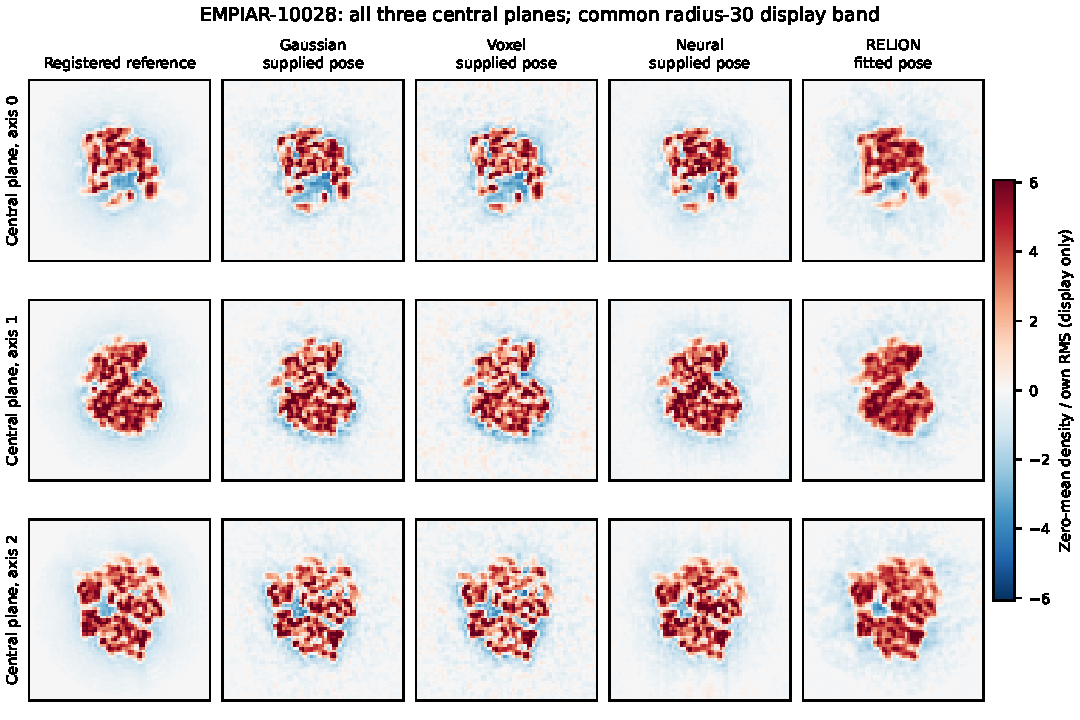
\includegraphics[width=\textwidth]{figures/reconstruction-slices-10028.pdf}
\caption{EMPIAR-10028: all three central planes of the registered reference and four existing reconstructions. Each square spans 482.4\,\AA. The display removes DC, retains a common radius-30 Fourier band, and divides each map by its own volumetric RMS; a pooled 99.5th-percentile absolute value fixes the common symmetric color range. This display normalization hides amplitude differences and is not used for FSC or intervals. Views are fixed array planes, not selected for agreement. Gaussian, voxel and neural estimates average the locked halves; RELION uses its previously evaluated map. Registration is pilot-derived. The 10076 reference represents Class A, not the heterogeneous consensus.}
\label{fig:slices10028}
\end{figure*}
\begin{figure*}[p]
\centering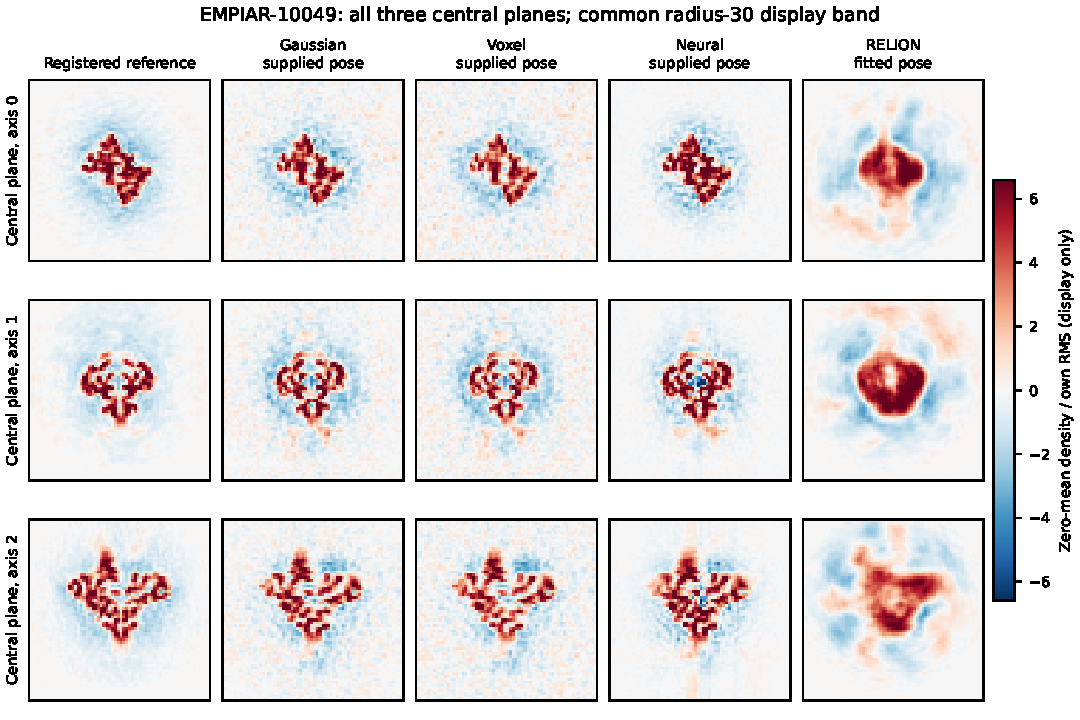
\includegraphics[width=\textwidth]{figures/reconstruction-slices-10049.pdf}
\caption{EMPIAR-10049: all three central planes of the registered reference and four existing reconstructions. Each square spans 236.16\,\AA. The display removes DC, retains a common radius-30 Fourier band, and divides each map by its own volumetric RMS; a pooled 99.5th-percentile absolute value fixes the common symmetric color range. This display normalization hides amplitude differences and is not used for FSC or intervals. Views are fixed array planes, not selected for agreement. Gaussian, voxel and neural estimates average the locked halves; RELION uses its previously evaluated map. Registration is pilot-derived. The 10076 reference represents Class A, not the heterogeneous consensus.}
\label{fig:slices10049}
\end{figure*}
\begin{figure*}[p]
\centering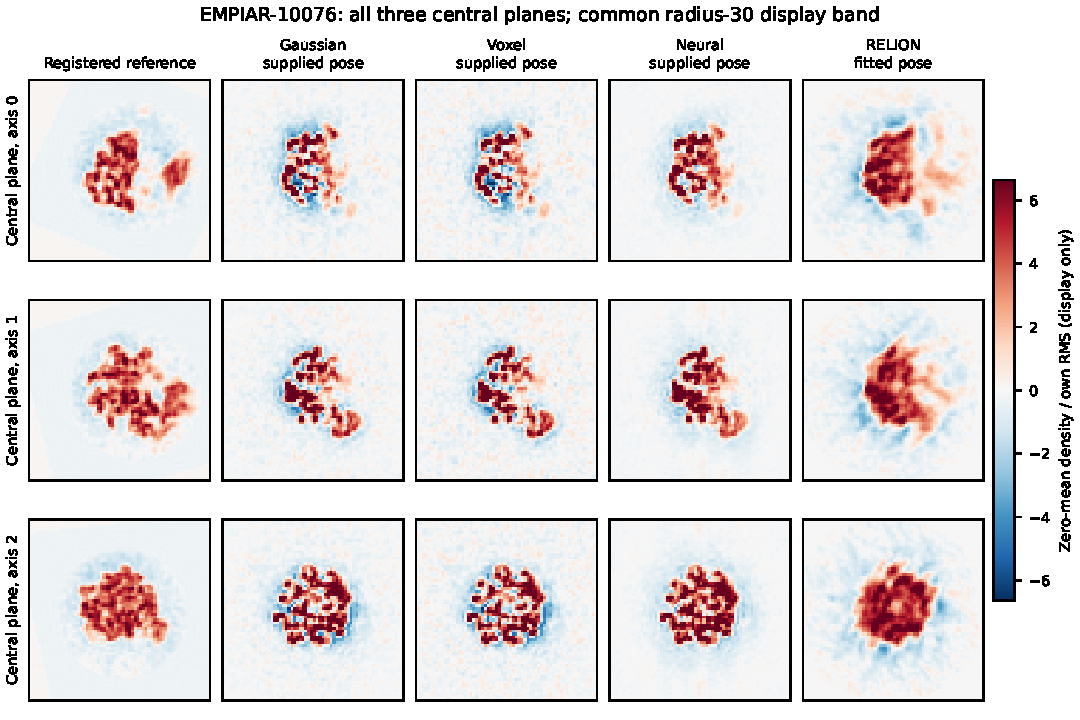
\includegraphics[width=\textwidth]{figures/reconstruction-slices-10076.pdf}
\caption{EMPIAR-10076: all three central planes of the registered reference and four existing reconstructions. Each square spans 419.2\,\AA. The display removes DC, retains a common radius-30 Fourier band, and divides each map by its own volumetric RMS; a pooled 99.5th-percentile absolute value fixes the common symmetric color range. This display normalization hides amplitude differences and is not used for FSC or intervals. Views are fixed array planes, not selected for agreement. Gaussian, voxel and neural estimates average the locked halves; RELION uses its previously evaluated map. Registration is pilot-derived. The 10076 reference represents Class A, not the heterogeneous consensus.}
\label{fig:slices10076}
\end{figure*}
